\documentclass[11pt]{article}
% shared/tex/preamble.tex
\usepackage[utf8]{inputenc}
\usepackage[T1]{fontenc}
\usepackage{microtype}
\usepackage{graphicx}
\usepackage{booktabs}
\usepackage{amsmath,amssymb}
\usepackage{xcolor}
\usepackage{tikz}
\usepackage{float}
\usepackage{siunitx}
\usepackage{hyperref}
\hypersetup{colorlinks=true, linkcolor=blue, citecolor=blue, urlcolor=blue}

% Define macros used across papers
\newcommand{\raphael}{\textit{Raphael}}


\title{Guardrail and Safety Frameworks for Clinical LLMs}
\author{Anthony Marra\\Villanova University}
\date{}

\begin{document}
\maketitle

\begin{abstract}
We describe a layered safety stack for clinical LLMs: retrieval grounding, close\-intent constraints, uncertainty calibration, and abstention. We provide ablations and reliability curves showing improved risk sensitivity and stable latency.
\end{abstract}

\section{Introduction}\section{Related Work}

\section{Methods}
\subsection{Uncertainty Calibration}\subsection{Deterministic Rules}\subsection{RAG Filtering}

\section{Results}
\begin{figure}[t]
\centering
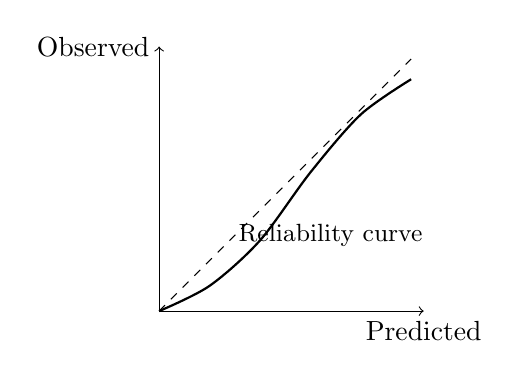
\begin{tikzpicture}[x=3.2cm,y=3.2cm]
  \draw[->] (0,0) -- (1.05,0) node[below] {Predicted};
  \draw[->] (0,0) -- (0,1.05) node[left] {Observed};
  \draw[dashed] (0,0) -- (1,1);
  \draw[thick] plot[smooth] coordinates {(0,0) (0.2,0.10) (0.4,0.28) (0.6,0.55) (0.8,0.78) (1,0.92)};
  \node at (0.68,0.30) {\small Reliability curve};
\end{tikzpicture}
\caption{Placeholder reliability diagram; replace with empirical plot.}
\label{fig:reliability}
\end{figure}

\section{Discussion}\section{Conclusion}

\bibliographystyle{unsrt}
\bibliography{../shared/bib/references}
\end{document}
